% Current IIoT data manuscript; C1 windows and full C2/C3 workloads.
% Match the user-designated Miao (TDSC 2025) paper's journal typography.
% Preserve the original Times font metrics across pdfLaTeX and XeTeX.
\RequirePackage[OT1]{fontenc}
\documentclass[10pt,journal]{IEEEtran}
\usepackage{graphicx,amsmath,amssymb,booktabs,array,url}
\usepackage{fontspec,xeCJK}
\setmainfont{Times New Roman}[Path=/mnt/c/Windows/Fonts/,UprightFont=times.ttf,BoldFont=timesbd.ttf,ItalicFont=timesi.ttf,BoldItalicFont=timesbi.ttf]
\setCJKmainfont{SimSun}[Path=/mnt/c/Windows/Fonts/,UprightFont=simsun.ttc,BoldFont=simhei.ttf,ItalicFont=simkai.ttf,BoldItalicFont=simhei.ttf,SmallCapsFont=simsun.ttc]
\setCJKsansfont{SimHei}[Path=/mnt/c/Windows/Fonts/,UprightFont=simhei.ttf]
\setCJKmonofont{SimSun}[Path=/mnt/c/Windows/Fonts/,UprightFont=simsun.ttc]
\renewcommand{\abstractname}{摘要}
\renewcommand{\IEEEkeywordsname}{关键词}
\renewcommand{\figurename}{图}
\renewcommand{\tablename}{表}
\renewcommand{\refname}{参考文献}
\linespread{1.10}
\usepackage[nocompress]{cite}
\interdisplaylinepenalty=2500
\usepackage[colorlinks=true,allcolors=blue]{hyperref}

\usepackage{xr}
\externaldocument[supp-]{supplementary}
\newcounter{algorithm}
\renewcommand{\thealgorithm}{\arabic{algorithm}}
\makeatletter
\newcommand{\fps@algorithm}{tbp}
\newcommand{\ftype@algorithm}{1}
\newcommand{\ext@algorithm}{loa}
\newcommand{\fnum@algorithm}{算法~\thealgorithm}
% Local ruled algorithm caption; leave IEEE table/figure captions untouched.
\newenvironment{algorithm}[1][t]{\@float{algorithm}[#1]%
  \long\def\@makecaption##1##2{%
    \par\hrule height .8pt\kern2pt
    {\normalfont\normalsize\noindent\textbf{##1:} ##2\par}%
    \kern2pt\hrule height .8pt\kern2pt}%
}{\end@float}
\makeatother
\newcommand{\ARC}{ARC-Audit}
\newcounter{proposition}
\newenvironment{proposition}[1]{%
  \refstepcounter{proposition}\par\smallskip\noindent
  \textbf{命题~\theproposition\ (#1). }\ignorespaces
}{\par\smallskip}
\newenvironment{claimproof}{\par\noindent\emph{证明：}\ignorespaces
}{\hfill\textit{证毕。}\par\smallskip}
\newcounter{algline}
\newcommand{\al}{\stepcounter{algline}\thealgline:}
\newcommand{\tabnote}[1]{\par\smallskip\parbox{\linewidth}{\footnotesize #1}}
\title{ARC-Audit：面向工业物联网数据的\\依赖感知审计与认证记录恢复}
\author{匿名作者}
\begin{document}
\bstctlcite{IEEEexample:BSTcontrol}
\maketitle
\begin{abstract}
共享压缩能够降低工业物联网（IIoT）数据的存储开销，但记录重建同时依赖局部编码和共享字典。因此，记录级审计与恢复需要确定解码所需的密文对象，并对所选对象进行认证。本文提出 ARC-Audit，通过认证恢复闭包连接公开完整性审计与认证记录恢复。其核心设计将公开可验证的依赖覆盖与授权恢复者的精确依赖发现相结合。认证布局将共享表示映射到加密页面，使公开验证者能够先合并充分覆盖的对象集合，再进行聚合认证。恢复者通过认证解密引用确定实际依赖，并利用经过验证的密文重建完整记录。受预算约束的密文保护支持该获取路径中的对象修复。本文分析表示正确性、依赖覆盖、聚合响应认证与返回记录真实性。两个 HAI 工作负载上的实验表明，共享表示减少云端存储，聚合审计减少应用层流量，同时相较对应对照增加构建与本地计算成本。精确依赖选择减少获取工作，并在被测失页案例中提高恢复成功率。恢复结果揭示了保护分配与请求所需对象的共同作用。
\end{abstract}
\begin{IEEEkeywords}
工业物联网，广义去重，公开完整性审计，认证记录恢复，依赖闭包，认证加密。
\end{IEEEkeywords}

\section{引言}\label{sec:introduction}
外包存储的工业物联网（IIoT）数据需要支持完整性验证和目标记录的可靠重建。共享压缩利用传感器字段和记录之间的重复结构：广义去重（GD）存储共享基及记录特有的引用与偏差~\cite{Talasila2019}，基于相似性的安全去重支持工业物联网数据的外包管理~\cite{Gao2024}。共享表示改变了数据访问单元：重建一条记录可能需要多个局部对象与共享对象，认证获取路径必须覆盖这些输入。

共享依赖使充分覆盖范围与实际解码需求存在区别。例如，设页 $p_0,p_1$ 包含某条记录的全部非字典输入，相关字典占据 $p_2,p_3$。若私有引用仅选中 $p_2$ 中的内容，实际输入位于 $\{p_0,p_1,p_2\}$，而覆盖整个字典还需要 $p_3$。此时，即使实际输入仍可获得，$p_3$ 不可用也会使完整字典覆盖失败。当多条记录引用 $p_2$ 时，联合请求还可以复用该页。因此，依赖模型需要同时表达对象选择所需的信息和跨记录的对象复用。

已有压缩、验证和保护机制分别处理这一问题的不同环节。压缩优化选择紧凑的数据表示~\cite{Hurst2024GreedyGD}；公开存储证明认证声明的挑战对象~\cite{ShachamWaters2013}；选择性访问系统优化数据获取~\cite{Taurone2024TREAT}；共享存储保护考虑公共块丢失的影响~\cite{Bhagwat2006Reliability}。面向记录的审计需要将选定对象的认证与目标记录完整解码路径的覆盖联系起来。因此，对象选择取决于表示布局、经过认证的引用以及各角色能够获得的信息。

ARC-Audit 通过\emph{认证恢复闭包}（authenticated recovery closure，ARC）描述这种联系，即足以重建目标记录的密文对象集合。所有者发布经过认证的寻址布局，同时加密完整解码内容。公开验证者据此覆盖相关字典、合并共享对象，并将结果绑定到新的聚合挑战。授权恢复者则先认证并解密引用，确定实际依赖后再获取其余对象。两种选择根据可用信息，将同一记录请求映射到不同的对象集合。

受预算约束的密文保护通过该认证获取路径提供修复。原始对象与 Reed--Solomon（RS）编码重建的对象均通过相同检查后进入完整记录解码。由此，共享布局连接存储表示、审计覆盖与恢复接受条件。

本文的主要贡献如下。
\begin{enumerate}
\item \emph{支持依赖寻址的加密共享表示。}将经全量序列化成本验证的字段分组与逻辑比特区间到密文页的认证映射相结合。该映射将逻辑记录依赖连接到经过认证的密文对象，同时将私有解码内容保留在加密数据中。
\item \emph{依赖感知的公开审计。}根据认证布局定义充分密文闭包，在聚合认证前合并重叠对象。公开布局无需解密引用即可提供充分覆盖，挑战绑定将目标记录连接到选定对象。
\item \emph{结合预算保护的精确认证恢复。}利用认证引用发现实际依赖，仅接受完整解码记录。密文 RS 保护层在序列化存储上限内提供经过验证的修复对象。
\end{enumerate}

两个 HAI 工作负载分别从存储与安全构建、公开审计的通信与计算，以及失页条件下的恢复评估上述设计。分组减少云端存储字节数，同时增加构建工作；公开闭包规划节省引用传输流量，同时覆盖更宽的对象集合；精确恢复减少获取和解码工作，并在未使用字典对象不可用的被测案例中提高成功率。
\section{相关工作}
\subsection{共享压缩与选择性访问}
共享压缩决定记录内容如何分布在局部编码和公共字典中。GD 通过共享基和各自的偏差重建数据块~\cite{Talasila2019}。GreedyGD 为压缩和直接分析选择基比特~\cite{Hurst2024GreedyGD}；EntroGD 将分析摘要与熵引导压缩相结合~\cite{Zhao2026EntroGD}。这些工作优化共享表示及其分析用途。ARC-Audit 通过认证记录区间和字典布局，将该表示连接到验证过程，使验证者能够在读取引用之前选择密文对象。

安全性与选择性访问进一步约束数据表示。安全相似性去重关注所有权与保密性，包括模糊消息锁定加密和所有权证明~\cite{Jiang2023FuzzyDedup}，以及工业物联网存储管理~\cite{Gao2024}。TREAT 将 GD、编码、重排和选择性获取相结合，用于分布式物联网查询~\cite{Taurone2024TREAT}。本文将公开寻址布局与私有解码内容分离，并对完整规范化记录的依赖进行认证。

\subsection{公开审计与可取回性}
公开存储验证围绕挑战选定的对象建立保证。PDP 检查外包数据的持有性~\cite{Ateniese2007PDP}；PoR 通过提取将挑战响应与数据恢复联系起来~\cite{Juels2007POR,ShachamWaters2013}。Bowers 等发展了 PoR 框架~\cite{Bowers2009PORTheory}，HAIL 则结合完整性检查与分布式冗余~\cite{Bowers2009HAIL}。动态 PDP 使用认证字典验证更新~\cite{Erway2009DPDP}。这些接口为各自规定的认证对象建立安全性质。近期，Yang 等通过压缩型 PDP 减少额外认证器存储，并采用线性通信的证明交换机制实现去中心化多云自审计~\cite{Yang2025CompressedPDP}。这里的压缩型 PDP 关注审计表示及其开销。ARC-Audit 则研究将认证对象与共享压缩记录重建连接起来的依赖选择。

共享数据审计也关注减少认证冗余和支持选择性验证。已有工作通过存储证明~\cite{Zheng2012POSD}、共享认证器~\cite{Tian2022SharedAudit}、客户端链下去重~\cite{Zhang2023BlockchainAudit}，以及减少密钥和认证器冗余~\cite{Miao2024SharedAudit}，结合审计与去重。隐私保护设计在加密数据去重和审计中保护文件所有权~\cite{Song2023EncryptedAudit}，并保护文件标签与审计证明隐私，同时采用基于身份的广播加密管理密钥~\cite{Zhang2025PrivacyAudit}。这些设计关注共享加密存储中的隐私与认证。

细粒度去重进一步连接审计与数据获取。Liu 等对用户内部及跨用户的密文和认证标签去重，并利用重构矩阵和 Bloom filter 获取分布式去重数据块~\cite{Liu2025FineGrained}。带仲裁的可搜索审计~\cite{Miao2025}、动态混合审计~\cite{Pan2026}和可更新多副本认证~\cite{Xu2026MPA}研究了相关的选择性与共享验证场景。ARC-Audit 显式建立验证对象与记录解码之间的联系：认证布局决定公开覆盖范围，经过认证的私有引用决定精确恢复输入。

认证数据结构将目录查询结果绑定到由数据源认证的信息~\cite{Goodrich2003ADS}。本文将该原则应用于布局及引用到共享基的对应关系。公开闭包规划从签名布局中获得充分覆盖；授权引用发现则先认证并解密引用所在位置，再选择更精确的集合。这一区别同时决定访问权限和通信成本。

\subsection{共享存储可靠性}
共享存储保护需要考虑记录对受保护对象的依赖。共享块丢失会影响多个逻辑对象。基于丢失影响的复制~\cite{Bhagwat2006Reliability}，以及对去重擦除编码存储的分析~\cite{Li2010Reliability}，说明了这种依赖结构的重要性。在系统层面，CDStore 将收敛分散与两阶段去重相结合，协调多云存储的可靠性、安全性和存储效率~\cite{Li2015CDStore}。Per-File Parity 将去重前校验与文件内、文件间恢复相结合~\cite{Wu2019PFP}；RepEC+ 结合复制、编码、选择和协同恢复~\cite{Zuo2022RepECPlus}。ARC-Audit 对完整密文对象采用标准 RS 编码~\cite{ReedSolomon1960}。实验固定编码和存储上限，改变页面分配方式以及认证恢复所要求的依赖集。

\section{系统模型与问题定义}\label{sec:model}
\subsection{参与角色与可信状态}
批次是独立配置、编码和认证的数据单元。\emph{数据所有者}对每个数据批次进行编码，并封装为不可变密文对象，生成审计标签并签署清单，同时保留批次级共享基和私有编码状态。\emph{云服务提供商}（CSP）存储密文对象、审计标签、公开参数、签名布局以及已部署的辅助保护文件。对象身份包括批次标识和页索引。快照指该批次签名清单所承诺的不可变编码状态。

\emph{公开验证者}持有所有者验证公钥和预期清单摘要，将其作为可信锚点；构造挑战前先认证公开布局与审计参数。\emph{授权恢复者}还持有批次解密能力，通过经认证的云端响应恢复记录。

签名清单绑定批次、公开布局、密文对象身份、长度与摘要、协议和审计参数。客户端保留完整的认证清单，其状态随对象数量增长。加密、清单签名和审计标签使用独立的秘密材料。跨批次请求按不可变批次划分，每个批次分别使用对应的可信锚点和密码上下文。

\subsection{威胁模型与安全目标}
CSP 可以遗漏对象、修改密文、替换元数据或标签，以及重放快照或响应。所有者诚实构建编码数据；验证者和恢复者使用真实的可信锚点及预置密钥执行规定算法。预期摘要标识请求的不可变版本。签名不可伪造性和抗碰撞哈希绑定保护该认证状态。

公开视图暴露记录数量、密文长度、组与比特布局、字典基数，以及请求的目标和对象。私有解码数值、常量、时间与标签内容、共享基和偏差均加密存储于逻辑容器中。内容保密性针对具有相同声明公开视图的输入定义，并基于第~\ref{sec:security}~节中的带关联数据的认证加密（AEAD）与密钥派生假设。

安全目标包括精确表示、以该公开视图为条件的内容保密性、认证依赖绑定、选定集合响应认证，以及返回记录真实性。第~\ref{sec:security}~节给出这些目标的前提与分析。恢复可用性通过请求期间可获得的认证原始对象和修复分片刻画。

\subsection{记录与密文对象}
数据表示将逻辑记录连接到承载其解码输入的密文页。规范化记录包含经精确缩放的过程值、索引、时间和标签。精确恢复指这些值在声明的模式下相等。对于批次 $b$，令 $F$ 为逻辑编码容器，将其划分为至多 $P_0=4068$ B 的明文切片 $F_p$。存储对象为
\begin{equation}\label{eq:cipher}
C_p=N_p\,\|\,\mathsf{Enc}_{k_b}(N_p,F_p,A_p),
\end{equation}
其中，$N_p$ 为 12 字节 nonce，$A_p$ 为关联数据，AEAD 输出包含 16 字节标签。因此，有效长度为 $\ell(p)=|F_p|+28\leq4096$ B。对象描述符和关联数据绑定身份与长度；不足整页的末尾切片保留实际长度。下文中的页指这一完整密文对象；$\mathcal P$ 为含批次信息的对象身份集合。

对于逻辑比特区间 $[a,a+w)$，公开映射为
\begin{equation}\label{eq:phi}
\Phi_{\mathcal L}(a,w)=
\left\{(b,p):\left\lfloor\frac{a}{8P_0}\right\rfloor
\leq p\leq\left\lfloor\frac{a+w-1}{8P_0}\right\rfloor\right\},
\end{equation}
并规定 $\Phi_{\mathcal L}(a,0)=\varnothing$。当比特区间跨越切片边界时，映射覆盖两侧对象。批次身份用于区分不同批次中相同的局部页索引。

\subsection{记录依赖与接受条件}
固定一个诚实构建的表示及其确定性解码器。精确依赖集 $\mathcal D_{\mathcal L}(i)$ 包含覆盖记录 $i$ 解码所需结构、引用、局部数据、标签和实际字典行的密文对象。公开恢复闭包 $K_{\mathcal L}(i)$ 则包含相关组的完整字典：
\begin{equation}\label{eq:sufficient-set}
\mathcal D_{\mathcal L}(i)\subseteq K_{\mathcal L}(i)\subseteq\mathcal P.
\end{equation}
两个集合对应同一固定解码器和页映射。精确依赖由该表示中的实际引用确定；公开闭包依据认证布局覆盖所有此类引用选择。

对于目标集合 $T$，公开审计认证 $U(T)=\bigcup_{i\in T}K_{\mathcal L}(i)$。授权恢复通过认证解密获取引用，并构造 $D(T)=\bigcup_{i\in T}\mathcal D_{\mathcal L}(i)$。因此，$K(i)$ 与 $\mathcal D(i)$ 描述单条记录的覆盖，$U(T)$ 与 $D(T)$ 合并请求中各目标对应的对象。公开验证者使用 $U(T)$，授权恢复者分两个阶段获取 $D(T)$。令 $\mathcal A$ 表示已取得承诺密文和认证明文的对象，包括成功修复的对象。记录恢复定义为
\begin{equation}\label{eq:record-recovery}
\mathsf{Rec}_i(\mathcal A)=
\mathbf1\{\mathcal D_{\mathcal L}(i)\subseteq\mathcal A
\ \land\ \widehat r_i=r_i\}.
\end{equation}
式~\eqref{eq:record-recovery}~定义恢复正确性。客户端仅接受经过认证的输入与完整解码结果，返回请求的全部记录或报告失败。Conservative 对照要求在解码前取得 $U(T)$。

审计接受要求元数据有效、上下文符合验证者预期，且所有涉及批次的响应均有效。恢复接受要求输入经过认证且完整解码成功。两类操作共享依赖语义，但对可用页面提出不同要求。

\begin{table}[t]\centering\small
\caption{加密审计与恢复的主要符号}\label{tab:notation}
\begin{tabular}{@{}l>{\raggedright\arraybackslash}p{.66\columnwidth}@{}}\toprule
符号 & 含义\\\midrule
$b$, $b_T$ & 批次身份；$T$ 涉及的批次数\\
$F,F_p,C_p$ & 逻辑容器、明文切片、密文对象\\
$k_b,N_p,A_p$ & 批次加密密钥、nonce、关联数据\\
$\mathcal L,\Phi_{\mathcal L}$ & 认证公开布局及比特区间映射\\
$\ell(p),\tau_p$ & 密文有效长度及公开审计标签\\
$\mathcal D(i),K(i)$ & 精确依赖及公开充分闭包\\
$D(T),U(T)$ & 精确依赖并集及审计闭包并集\\
$\pi=(\sigma,\boldsymbol\mu)$ & 聚合审计响应\\
$\beta,B_{\rm side}$ & 保护预算比例；\newline 辅助保护文件计费字节数\\\bottomrule
\end{tabular}\end{table}

\begin{figure*}[t]\centering
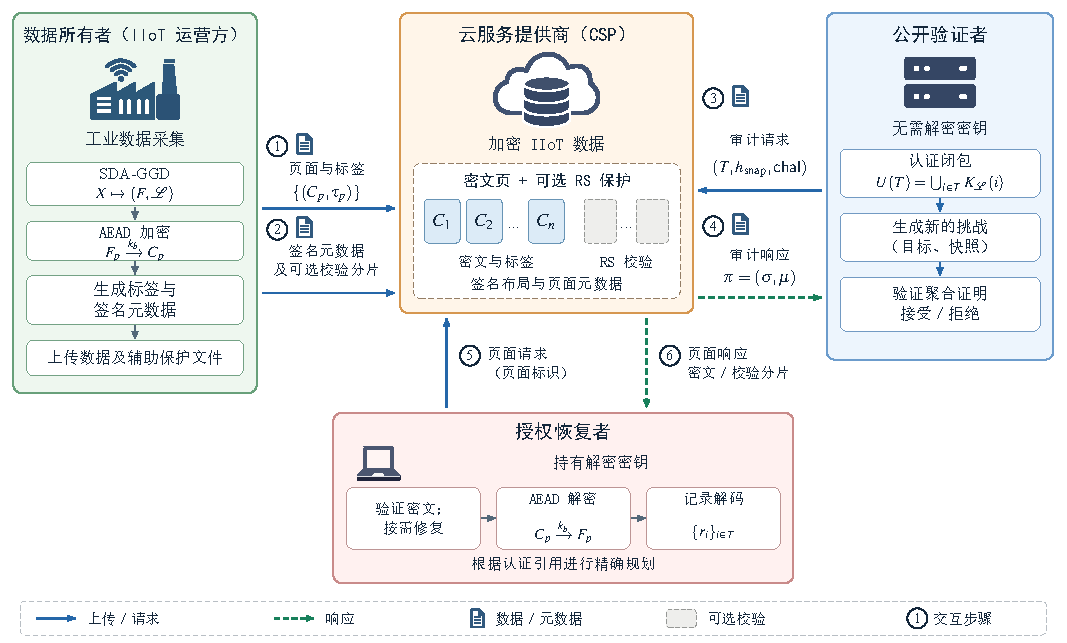
\includegraphics[width=\textwidth]{figures/cn/architecture.pdf}
\caption{ARC-Audit 的系统架构与数据流。公开审计根据经认证的布局推导 $U(T)$。授权恢复认证并解密引用以确定实际依赖；原始密文和修复密文均需在解码前通过相同检查。带密钥的箭头表示使用批次密钥 $k_b$ 的 AEAD 封装与解封，其中包含 nonce 和关联数据处理。}
\label{fig:architecture}\end{figure*}

\section{ARC-Audit 方案设计}\label{sec:design}
\subsection{方案概述}
ARC-Audit 通过认证依赖布局连接对象选择、响应认证和记录重建（图~\ref{fig:architecture}）。构建阶段对记录分组和编码，加密可寻址页面并认证其布局。公开依赖规划选择并合并充分覆盖所需的对象，聚合审计认证这些对象对新鲜挑战的线性响应。授权恢复通过认证引用发现实际依赖，并在输入验证与完整解码后返回记录。

保护层通过同一验证访问接口，为恢复所需对象提供经过认证的修复。下文依次说明这些操作及其资源核算。

\subsection{经全量成本验证的共享表示}\label{sec:c1}
字段分组需要在减少编码大小的同时，保留依赖规划所需的位置信息。本文将字段分组 GD 构造记为 SDA-GGD：以样本收益排列候选合并顺序，再以全量序列化成本决定是否接受。所得布局给出记录区间与字典范围，使验证者能够在读取引用前选择页面。

\emph{编码与序列化成本。}为每个字段声明精确的十进制缩放因子和整数位宽。常量仅存储一次，其余字段划分为若干组。对于总位宽为 $L_g$ 的组 $G$，选择 $k$ 个基比特位置，令 $M_g$ 为观测到的不同共享基数量。其余 $L_g-k$ 个位置构成偏差。每条记录存储长度为 $b_g=\lceil\log_2M_g\rceil$ 比特的固定宽度基标识及偏差，字典存储共享基。

对于 $n$ 条记录，组的序列化成本为
\begin{equation}\label{eq:cost}
\begin{split}
C(G)={}&C_{\mathrm{hdr}}(G,k)+\lceil M_gk/8\rceil+\lceil nb_g/8\rceil\\
 &+\lceil n(L_g-k)/8\rceil,
\end{split}
\end{equation}
其中，$C_{\mathrm{hdr}}(G,k)=11+2|G|+2k$ 字节用于存储组模式、字段标识和基比特位置。RAW 组的成本为 $C_{\mathrm{hdr}}(G,0)+\lceil nL_g/8\rceil$。各数据流独立序列化，因此需要分别取整。完整容器成本为 $C_0+\sum_G C(G)$，其中 $C_0$ 包括固定模式、常量、时间与标签表示以及全局头部。

\emph{组内配置。}配置器按经验二元熵升序对局部比特位置进行稳定排序，并测试长度为 $k=0,1,\ldots,L_g$ 的前缀。当 $M_g=n$ 时停止。在可行候选中，选择按字节取整后成本最小的配置；成本相同时选择较早的前缀。若 RAW 成本不高于该 GD 候选，则选择 RAW。合并组按顺序拼接字段序列；熵相同时保留该局部比特顺序。测试配置依据序列化成本在这些候选之间选择。

\emph{样本排序与全量确认。}初始化时，每个非常量字段构成一个活动组。固定样本给出联合字节收益 $\widehat\Delta=C_m(G_a)+C_m(G_b)-C_m(G_a\mathbin{\|}G_b)$，其中 $C_m$ 在相同样本行上配置并测量各组，$\|$ 表示有序字段拼接。仅将正估计收益加入队列。在全量确认前刷新候选，并丢弃过期版本。
合并 $(G_a,G_b)$ 前，编码器在全部输入记录上重新配置组合组并计算
\begin{equation}
\Delta_{\mathrm{full}}=C(G_a)+C(G_b)-C(G_a\mathbin{\|}G_b).
\end{equation}
仅当完整序列化字节收益和载荷收益均为正时才接受合并。更新受影响候选，直至队列为空。RAW 回退计入配置的实际字节成本。算法~\ref{alg:grouping}~以精确记录 $X$、模式 $\Sigma$ 和固定样本索引 $I$ 为输入。辅助函数 $\operatorname{Config}(X,G)$ 选择组配置，包括 RAW 回退。$C(G;c)$ 表示配置 $c$ 下的序列化成本，$C_{\mathrm{pay}}(G;c)$ 表示不含组头部、按字节取整后的载荷成本。省略 $c$ 时指当前配置。$\operatorname{SampleGain}$ 返回样本收益和合并配置；仅凭样本估计不能决定接受合并。

算法~\ref{alg:grouping}~中，$J$ 存储被拒绝的带版本组对，$d_e$ 记录最多 $d_{\max}=8$ 次的重新入队次数，$\operatorname{TopGain}$ 返回队首存储的收益，空队列返回 $-\infty$。补充材料第~\ref*{supp-sec:configuration}~节规定版本检查与同分处理规则。

\begin{algorithm}[t]\centering\normalsize\setcounter{algline}{0}
\caption{全量成本验证分组}\label{alg:grouping}
\begin{tabular}{@{}r@{\enspace} >{\raggedright\arraybackslash}p{.88\columnwidth}@{}}
\multicolumn{2}{@{}p{\columnwidth}@{}}{\textbf{输入：}记录 $X$，模式 $\Sigma$，样本索引 $I$。}\\
\multicolumn{2}{@{}p{\columnwidth}@{}}{\textbf{输出：}逻辑容器 $F$ 和公开布局 $\mathcal L$。}\\
\al & $\mathcal G\gets$ 由单个非常量字段组成的组。\\
\al & 在 $X$ 和 $X_I$ 上配置 $\mathcal G$；$J\gets\varnothing$。\\
\al & $Q\gets$ 样本收益为正的组对；初始化 $d_e=0$。\\
\al & \textbf{当} $Q\neq\varnothing$ \textbf{时执行}\\
\al & \hspace*{1em}$e=(G_a,G_b,\text{versions})\gets\operatorname{PopMax}(Q)$。\\
\al & \hspace*{1em}\textbf{若} $e$ 过期或 $e\in J$，\textbf{继续}。\\
\al & \hspace*{1em}$(\widehat\Delta,\widehat c)\gets\operatorname{SampleGain}(X_I,G_a,G_b)$。\\
\al & \hspace*{1em}\textbf{若} $\widehat\Delta\leq0$，将 $e$ 加入 $J$；\textbf{继续}。\\
\al & \hspace*{1em}\textbf{若} $\operatorname{TopGain}(Q)>\widehat\Delta$ 且 $d_e<d_{\max}$，\textbf{则}\\
\al & \hspace*{2em}$d_e\gets d_e+1$；以 $\widehat\Delta$ 将 $e$ 重新入队；\textbf{继续}。\\
\al & \hspace*{1em}\textbf{结束条件分支}\\
\al & \hspace*{1em}$G_c\gets G_a\mathbin{\|}G_b$；$c\gets\operatorname{Config}(X,G_c)$。\\
\al & \hspace*{1em}$\Delta_{\mathrm{full}}\gets C(G_a)+C(G_b)-C(G_c;c)$。\\
\al & \hspace*{1em}$\Delta_P\gets C_{\mathrm{pay}}(G_a)+C_{\mathrm{pay}}(G_b)-C_{\mathrm{pay}}(G_c;c)$。\\
\al & \hspace*{1em}\textbf{若} $\Delta_{\mathrm{full}}>0$ 且 $\Delta_P>0$，\textbf{则}\\
\al & \hspace*{2em}用配置为 $(c,\widehat c)$ 的 $G_c$ 替换 $\mathcal G$ 中的 $G_a,G_b$。\\
\al & \hspace*{2em}使旧组条目失效；将收益为正的新建／有效组对入队。\\
\al & \hspace*{1em}\textbf{否则}将 $e$ 加入 $J$。\\
\al & \hspace*{1em}\textbf{结束条件分支}\\
\al & \textbf{结束循环}\\
\al & $(F,\mathcal L)\gets\operatorname{Serialize}(X,\Sigma,\mathcal G)$。\\
\al & \textbf{返回} $(F,\mathcal L)$。\\\bottomrule
\end{tabular}\end{algorithm}

\begin{proposition}{经确认的逻辑成本下降}\label{prop:cost}
每次接受合并都会严格降低经检查的逻辑序列化成本及其载荷成本。从 $g_0$ 个活动组开始，最多接受 $g_0-1$ 次合并。
\end{proposition}
\begin{claimproof}
算法~\ref{alg:grouping}~仅接受全量序列化收益和载荷收益均为正的候选。未改变的组保持原有成本，容器固定部分不变。每次接受合并用一个组替换两个组。被拒绝的带版本组对被记录，过期项被丢弃，有限的重新入队次数保证两次合并之间的处理终止。
\end{claimproof}
式~\eqref{eq:cloud-cost}~中的实测安全成本还包括加密封装、标签和公开清单。RQ1 将该最终成本与分组目标分别评估。

\subsection{页面加密与认证布局}\label{sec:seal}
页面加密将依赖定位所需信息与解码所需数值分开处理。公开布局包含数据流位置、位宽、模式、基比特位置、字典基数和记录数量。完整逻辑容器存储私有解码头部、数值及编码记录。布局支持式~\eqref{eq:phi}；数值常量和私有字段值保留在加密切片中。

每次构建时，所有者生成新的 256 比特批次标识 $b$ 和随机加密主秘密。HKDF-SHA256 以 $b$ 为盐值、\texttt{ARC/ENC/v1} 为上下文派生 $k_b$~\cite{RFC5869}。nonce 为局部页索引的 96 比特编码，因此同一批次密钥下各页的 nonce 不同。AES-256-GCM 按式~\eqref{eq:cipher}~封装各切片~\cite{RFC5116}。关联数据是协议、所有者域、批次、对象身份、编解码器和明文长度的规范编码。这些字段保留在公开描述符中。

描述符还记录完整密文的长度和哈希。审计标签身份绑定该描述符及公开参数指纹。创建密文对象和标签后，所有者使用 Ed25519 签署规范清单，其中包含描述符、公开布局、参数和标签文件摘要。清单摘要与签名公钥构成预置可信锚点。该顺序将标签绑定到不可变对象，并将清单绑定到已生成的标签，避免摘要循环依赖。算法~\ref{alg:seal}~概括了这一构造。

\begin{algorithm}[t]\centering\normalsize\setcounter{algline}{0}
\caption{数据批次封装}\label{alg:seal}
\begin{tabular}{@{}r@{\enspace} >{\raggedright\arraybackslash}p{.88\columnwidth}@{}}
\multicolumn{2}{@{}p{\columnwidth}@{}}{\textbf{输入：}逻辑容器 $F$，公开布局 $\mathcal L$，所有者域。}\\
\multicolumn{2}{@{}p{\columnwidth}@{}}{\textbf{输出：}密文对象、审计标签、签名清单及客户端可信锚点。}\\
\al & 生成新的批次 $b$ 和加密主秘密；派生 $k_b$。\\
\al & 生成独立审计秘密 $x$、公开参数 $\mathsf{pp}$ 和清单签名密钥。\\
\al & \textbf{对每个}不超过 4068 B 的切片 $F_p$ \textbf{执行}\\
\al & \hspace*{1em}$N_p\gets\operatorname{Encode}_{96}(p)$；构造认证头部 $A_p$。\\
\al & \hspace*{1em}$C_p\gets N_p\|\mathsf{Enc}_{k_b}(N_p,F_p,A_p)$。\\
\al & \hspace*{1em}$d_p\gets(A_p,|C_p|,\mathsf{Hash}(C_p))$。\\
\al & \hspace*{1em}$\tau_p\gets\operatorname{Tag}(x,\mathsf{pp},d_p,C_p)$。\\
\al & \textbf{结束循环}\\
\al & $M\gets\operatorname{Manifest}(b,\mathcal L,\{d_p\},\mathsf{pp},\mathsf{Hash}(\{\tau_p\}))$。\\
\al & 签署规范清单 $M$；预置签名公钥和 $\mathsf{Hash}(M)$ 作为可信锚点。\\
\al & 保留批次级私有编码状态和解密能力。\\
\al & \textbf{返回} $\{C_p\},\{\tau_p\},M$、签名和可信锚点。\\\bottomrule
\end{tabular}\end{algorithm}

\subsection{认证恢复闭包}\label{sec:c2}
公开规划以目标集 $T$ 和认证布局为输入，返回对象并集 $U(T)$。通过包含每个相关组的完整字典，该过程覆盖未知引用，仅凭布局即可得到充分覆盖。令 $S$ 覆盖私有结构元数据，$R_g(i)$ 为记录 $i$ 在组 $g$ 中的引用区间，$V_g(i)$ 为其偏差或 RAW 内容，$L(i)$ 为其标签；这些集合均经 $\Phi_{\mathcal L}$ 映射。令 $\mathcal P_g^{\rm dict}$ 包含 GD 组映射后的全部字典页。定义
\begin{equation}\label{eq:closure}
K(i)=S\cup L(i)\cup\bigcup_g
\bigl(R_g(i)\cup V_g(i)\cup\mathcal P_g^{\rm dict}\bigr).
\end{equation}
对于 RAW 组，引用项和字典项为空。私有结构包含解码器所需模式和格式信息。标签覆盖选取目标的标签比特。每个区间包含与其相交的所有密文对象，即使某一对象混合存储了多个逻辑流的内容。

验证者依据公开布局构造 $K(i)$。纳入完整组字典可以覆盖任何有效 BaseID 所选中的字典行。授权路径则认证并解密 $S$ 和引用页，在承诺位置读取各 BaseID，检查其范围，并映射被引用的字典行。这些行与 $S$、引用、局部内容和标签共同构成 $\mathcal D(i)$。

公开请求以 $U(T)=\bigcup_{i\in T}K(i)$ 对共享对象去重并合并。对于密文长度 $\ell(p)$，对象并集与分别执行且不使用缓存的闭包访问，其逻辑读取字节数分别为
\begin{equation}\label{eq:reads}
B_U=\sum_{p\in U(T)}\ell(p),\qquad
B_N=\sum_{i\in T}\sum_{p\in K(i)}\ell(p).
\end{equation}
请求缓存也可以将分别遍历的读取范围缩减为唯一对象集合。对照实验将这种读取复用效果与证明聚合区分。对于多个数据批次，使用包含批次信息的身份分别计算目标与并集，再在请求层面合并结果。

\subsection{基于新鲜挑战的公开聚合审计}\label{sec:audit}
聚合审计认证验证者选定闭包上的线性响应。将目标、快照和选定对象绑定到新鲜挑战，使响应对应于请求记录及其版本。

每个完整密文对象采用虚拟零填充，编码为 $s=133$ 个 31 B 的小端扇区。对于 BLS12-381 的标量阶 $q$，扇区整数满足 $m_{p,j}<2^{248}<q$。因此，nonce、加密载荷和 AEAD 标签均受到覆盖；签名有效长度决定尾部填充的去除。

所有者选择秘密 $x$，公开 $Y=xg_2$，并在 $\mathbb G_1$ 中计算标签，配对为 $e:\mathbb G_1\times\mathbb G_2\to\mathbb G_T$：
\begin{equation}\label{eq:tag}
\tau_p=x\left(H(W_p)+\sum_{j=1}^{s}m_{p,j}u_j\right).
\end{equation}
$W_p$ 绑定完整密文描述符和参数指纹。基点 $u_j$ 与描述符哈希 $H$ 使用域分离的哈希到曲线操作~\cite{RFC9380}。该构造遵循 Shacham--Waters 的线性公开认证结构~\cite{ShachamWaters2013}。

对于每个批次请求，验证者生成新的 256 比特 nonce。规范挑战绑定快照、参数、目标、页集合、请求策略和会话。将该上下文的规范编码与页索引、重试计数器共同哈希，再进行标量约简并拒绝零值，得到 $\nu_p\in\mathbb F_q^*$。补充材料第~\ref*{supp-sec:backend-interface}~节规定域分离与编码。

\mbox{CSP 返回}
\begin{equation}\label{eq:aggregate}
\sigma=\sum_{p\in U}\nu_p\tau_p,\qquad
\mu_j=\sum_{p\in U}\nu_pm_{p,j}\pmod q.
\end{equation}
在检查上下文、格式、曲线点、子群、标量范围和维度后，验证者检验
\begin{equation}\label{eq:pairing}
e(\sigma,g_2)=e\left(\sum_{p\in U}\nu_pH(W_p)+\sum_j\mu_ju_j,Y\right).
\end{equation}
验证者保留自行确定的预期页集合。公开参数排除无效基点与单位元，响应必须同时满足解析规则和式~\eqref{eq:pairing}。算法~\ref{alg:audit}~给出公开审计流程。

\begin{algorithm}[t]\centering\normalsize\setcounter{algline}{0}
\caption{公开闭包审计}\label{alg:audit}
\begin{tabular}{@{}r@{\enspace} >{\raggedright\arraybackslash}p{.88\columnwidth}@{}}
\multicolumn{2}{@{}p{\columnwidth}@{}}{\textbf{输入：}目标 $T$，对应清单和可信锚点，公开审计参数。}\\
\multicolumn{2}{@{}p{\columnwidth}@{}}{\textbf{输出：}\texttt{ACCEPT} 或 \texttt{REJECT}。}\\
\al & 验证者按不可变批次划分 $T$。\\
\al & \textbf{对每个}涉及的批次 $b$ \textbf{执行}\\
\al & \hspace*{1em}依据可信锚点认证清单；验证 $T_b$ 与参数。\\
\al & \hspace*{1em}\textbf{若}验证失败，\textbf{返回} \texttt{REJECT}。\\
\al & \hspace*{1em}$U_b\gets\operatorname{SortUnique}(\bigcup_{i\in T_b}K_{\mathcal L_b}(i))$。\\
\al & \hspace*{1em}生成新的 nonce；绑定预期快照、请求、$T_b$ 和 $U_b$。\\
\al & \hspace*{1em}派生 $\nu_p\in\mathbb F_q^*$；发送挑战并保留预期上下文。\\
\al & \hspace*{1em}CSP 读取唯一 $C_p$（$p\in U_b$），按式~\eqref{eq:aggregate}~响应。\\
\al & \hspace*{1em}验证者检查响应格式、上下文、编码及式~\eqref{eq:pairing}。\\
\al & \hspace*{1em}\textbf{若}任一检查失败，\textbf{返回} \texttt{REJECT}。\\
\al & \textbf{结束循环}\\
\al & \textbf{返回} \texttt{ACCEPT}。\\\bottomrule
\end{tabular}\end{algorithm}

在固定扇区划分下，每个批次的聚合证明占 4310 B。因此，涉及 $b_T$ 个批次的请求包含 $4310b_T$ 字节证明，另需计入声明与挑战。第~\ref{sec:eval}~节按实际应用层封装，将该公开接口与授权引用发现和公开下载进行比较。

对于固定挑战，逐页证明对照为每个 $p$ 返回 $(\nu_p\tau_p,(\nu_pm_{p,j})_j)$，并验证相应的单页方程。因此，聚合响应和逐页响应使用相同选定页及新生成的系数。补充材料第~\ref*{supp-sec:wire-format}~节给出序列化细节。

\subsection{精确认证记录恢复}\label{sec:c3}
精确恢复分为两个认证阶段：先发现用于确定依赖的引用，再获取这些依赖以完成解码。恢复者验证清单、版本可信锚点及辅助保护文件的绑定。首先获取用于解析目标依赖的结构与引用密文，检查各对象身份、长度和承诺摘要，并执行 AEAD 认证解密。此后才能解析私有结构和 BaseID，构造精确依赖。其余字典行、偏差、RAW 内容及目标标签经同一验证路径获取。

请求本地缓存保留经认证的内容。私有解码器的格式与认证公开布局进行一致性检查；每次比特读取都必须落在已验证明文中。取得全部必需输入后，确定性解码器重建每条请求的规范化记录。认证、引用范围、格式或解码检查失败均返回 $\bot$。算法~\ref{alg:recovery}~针对单个批次；多批次恢复对涉及的各批次执行相同过程。

辅助函数 $\operatorname{VerifiedOpen}$ 以对象身份和认证批次上下文为输入，直接或通过受保护获取接口取得承诺密文，验证描述符后进行认证解密。该函数返回验证通过的明文或 $\bot$，仅缓存经过验证的密文与认证明文。

\begin{algorithm}[t]\centering\normalsize\setcounter{algline}{0}
\caption{精确认证记录恢复}\label{alg:recovery}
\begin{tabular}{@{}r@{\enspace} >{\raggedright\arraybackslash}p{.88\columnwidth}@{}}
\multicolumn{2}{@{}p{\columnwidth}@{}}{\textbf{输入：}清单与可信锚点、解密能力、目标 $T$、云端获取接口、可选的签名辅助保护文件。}\\
\multicolumn{2}{@{}p{\columnwidth}@{}}{\textbf{输出：}完整记录 $\{r_i\}_{i\in T}$ 或 $\bot$。}\\
\al & 认证清单和辅助保护文件；验证目标与绑定关系。\\
\al & \textbf{若}验证失败，\textbf{返回} $\bot$。\\
\al & $I\gets S\cup\bigcup_{i\in T,g}R_g(i)$；$\mathcal C\gets\varnothing$。\\
\al & \textbf{对每个} $p\in I$ \textbf{执行}\\
\al & \hspace*{1em}$\mathcal C[p]\gets\operatorname{VerifiedOpen}(p)$；失败则\textbf{返回} $\bot$。\\
\al & \textbf{结束循环}\\
\al & 解析认证引用；检查范围；推导 $D(T)$。\\
\al & \textbf{对每个} $p\in D(T)\setminus\operatorname{dom}(\mathcal C)$ \textbf{执行}\\
\al & \hspace*{1em}$\mathcal C[p]\gets\operatorname{VerifiedOpen}(p)$；失败则\textbf{返回} $\bot$。\\
\al & \textbf{结束循环}\\
\al & 验证私有／公开格式；从 $\mathcal C$ 解码完整记录。\\
\al & \textbf{若}解析或解码失败，\textbf{返回} $\bot$。\\
\al & \textbf{返回} $\{r_i\}_{i\in T}$。\\\bottomrule
\end{tabular}\end{algorithm}

Conservative 对照将第 3 行的 $I$ 替换为 $U(T)$，后续认证与解码相同。因此，即使某个未使用字典对象不可用，只要实际解码输入可直接获取或通过修复取得，Exact 恢复仍可执行。

\subsection{预算约束下的密文保护}\label{sec:protection}
共享页可能被多条记录共同需要，因此保护分配影响哪些解码路径仍然可用。ARC-Audit 在共同存储上限内修复选定密文对象，并在解码前验证每个修复结果。

GF$(256)$ 上的系统型 RS$(10,8)$ 辅助保护文件将八个密文对象组成一组，每个条带存储两个校验分片。原始对象保持原位。较短对象虚拟补零至 4096 B；不完整条带使用声明的虚拟零槽位。校验在包含 nonce 和 AEAD 标签字节的密文上计算。签名辅助保护文件绑定父快照、编码维度、条带成员和校验摘要。

Dictionary 将包含字典的页排在其他对象之前；Uniform 使用带种子的随机排列；FrequencyD 按参考记录集合中的依赖频次排序对象。三种排序采用相同条带数量，确保每个生成的辅助保护文件均满足同一批次上限：
\begin{equation}\label{eq:budget}
B_{\rm side,b}\leq\left\lfloor\beta B_{\rm cipher,b}\right\rfloor.
\end{equation}
保护预算决定获得保护的密文条带数量，RS$(10,8)$ 则规定每个准入条带内部的冗余配置。计费内容包括校验分片、序列化清单、签名、签名公钥和摘要锚点。实验使用 $\beta=0.10$，并设置零冗余的 NoEC 对照。条带数量和上限相同，但实际序列化保护文件长度可以不同。

受保护获取首先检查原始对象。若不可用，恢复者从其条带收集互不相同且经过认证的存活原始／校验槽位。八个有效槽位即可执行 RS 重建。每个重建的真实对象按签名长度截断，并在进入缓存前与原始密文摘要核对；随后进行 AEAD 认证，再解码记录。同一辅助函数处理引用发现阶段或最终精确依赖集所需的修复。

\subsection{计算与存储成本核算}\label{sec:accounting}
令 $N$ 为一个批次中的密文对象数，$u=|U(T)|$。除常驻认证元数据外，直接枚举闭包需要期望 $O(\sum_{i\in T}|K(i)|)$ 次集合插入工作和 $O(u)$ 的唯一对象状态。分组成本为实际执行的样本配置、全量配置与队列更新成本之和。每次接受合并都会减少活动组数量。

标签生成处理 $Ns$ 个扇区。生成证明累加 $us$ 个域乘积和 $u$ 个加权标签；验证形成 $u$ 个描述符哈希项和 $s$ 个扇区基点项，随后执行两次配对。请求级成本跨涉及的批次累加。固定的单批次证明大小，与页集合挑战材料以及随 $N$ 增长的清单同时存在。

对于不含辅助保护文件的编码数据，云端存储字节数为
\begin{equation}\label{eq:cloud-cost}
B_{\rm cloud}=B_{\rm cipher}+B_{\rm tags}+B_{\rm manifest},
\end{equation}
其中，$B_{\rm tags}=48N$，签名清单包含公开参数。AEAD 在 $B_{\rm cipher}$ 中贡献 $28N$ 字节。所有者侧共享基字节数和总私有状态单独统计。部署辅助保护文件会增加云端文件；保护状态核算还计入预置可信锚点，从而区分云端存储与客户端预置状态。

应用层流量包括声明、挑战、使用时的第一阶段材料及响应。初始化认证并解析清单和参数；请求计时测量在该上下文中执行指定操作的时间。恢复计时覆盖获取／修复、认证、解密和解码。服务器读取与应用层回复分别核算，因为修复一个返回页可能需要读取多个分片。

\section{安全性与可恢复性分析}\label{sec:security}
本节首先建立精确表示、充分依赖覆盖以及对象认证绑定，随后分析内容保密性、聚合审计响应与返回记录真实性。最后，恢复条件将这些保证连接到可用原始对象和修复分片。分组成本性质已由命题~\ref{prop:cost}~给出。

假设编码数据诚实构建、模式算术精确、组配置有效、客户端可信锚点真实，且预置解密能力正确。密码学前提包括签名不可伪造性、哈希抗碰撞性、安全密钥派生、遵守 nonce 使用条件的 AEAD 安全性，以及下述选定集合响应认证假设。表~\ref{tab:security}~概括各前提的作用。

\begin{table}[t]\centering\small
\caption{安全性质及其前提}\label{tab:security}
\begin{tabular}{@{}>{\raggedright\arraybackslash}p{.39\columnwidth}>{\raggedright\arraybackslash}p{.55\columnwidth}@{}}\toprule
性质 & 主要前提\\\midrule
精确表示 & 模式有效、比特互补划分、解码器正确\\
内容保密性 & 公开视图相同、安全派生、nonce 唯一、AEAD 保密性\\
闭包充分性 & 认证布局与完整比特区间映射\\
依赖绑定 & 清单签名、可信摘要、对象哈希绑定\\
选定集合响应认证 & 紧凑接口的响应认证假设\\
返回记录真实性 & 密文绑定、认证解密、精确解码\\
条件恢复 & 必需原始对象或足够的认证修复槽位\\
保护上限 & 完整序列化辅助保护文件的准入检查\\\bottomrule
\end{tabular}\end{table}

\subsection{表示正确性}\label{sec:representation-proof}
精确重建依据共享基与偏差比特位置的互补关系。对于已配置字段组，令 $I_g$ 包含选定的基比特位置，$J_g$ 为其补集。记录的组比特串满足 $x_{i,g}[I_g]=B_{g,\mathrm{ID}_{i,g}}$ 和 $x_{i,g}[J_g]=d_{i,g}$。存储的标识选择准确的字典行。将其比特与偏差分别放回互补位置，即可重建 $x_{i,g}$。根据声明的位宽和精确十进制缩放关系进行逆变换，得到字段值；RAW、常量、时间与标签遵循各自声明的表示。

\begin{proposition}{精确表示}\label{prop:representation}
对于诚实配置的批次，对其完好且必需的密文对象进行认证解密和解码，可以返回完整的规范化记录。
\end{proposition}
\begin{claimproof}
AEAD 正确性保证在绑定的 nonce 和关联数据下返回原始切片，其逻辑位置重新组成解码器输入。互补比特重建得到各非常量字段组，RAW 与元数据解码提供其余数值。完整字段覆盖由此得到规范化记录的全部组成部分。
\end{claimproof}

\subsection{闭包充分性与共享对象复用}\label{sec:closure-proof}
公开闭包需要覆盖实际引用选定的每个对象。下述包含关系将公开规划与解码输入连接起来。
\begin{proposition}{充分的密文覆盖}\label{prop:closure}
对于每个有效目标，$\mathcal D(i)\subseteq K(i)$；因此，对于任意有效目标集 $T$，都有 $D(T)\subseteq U(T)$。
\end{proposition}
\begin{claimproof}
两个集合均包含必需的结构、引用、局部内容和标签。对于 GD 组，精确路径选择一个有效字典行；与该行相交的所有对象均属于 $K(i)$ 中映射后的完整字典范围。RAW 组不增加字典依赖。式~\eqref{eq:phi}~的映射包含与逻辑比特区间相交的每个对象。对组和目标取并集保持包含关系。
\end{claimproof}

令 $a_p=|\{i\in T:p\in K(i)\}|$，则
\begin{equation}\label{eq:reuse}
B_N-B_U=\sum_{p\in U(T)}(a_p-1)\ell(p)\geq0.
\end{equation}
该恒等式说明无缓存读取的节省来自对象重叠，也解释了为什么具有完整请求缓存的分别遍历能够达到与并集相同的读取量。聚合减少选定集合的重复响应，是另一项机制；实验在相同挑战和页面下对其评估。

\subsection{认证依赖绑定}\label{sec:binding}
清单签名和可信摘要认证预期布局与密文描述符。因此，公开选择遵循所有者承诺的映射。精确选择还认证密文引用字节，在绑定的批次密钥和关联数据下解密，并在计算字典行之前检查各 BaseID。私有／公开格式一致性检查，使这种解释与对象获取所用布局一致。

定义 $\mathsf{BadBind}$ 为接受与预期签名快照不一致的元数据或对象描述符，$\mathsf{BadHash}$ 为接受与承诺密文或校验摘要对应的不同字节。在真实可信锚点下，签名不可伪造性和抗碰撞性约束这些事件的概率。若这些事件均不发生，替换不同引用、页面、快照或条带就无法改变被接受的解码输入。直接获取及 RS 重建后都检查原始密文摘要。

\subsection{公开视图下的内容保密性}\label{sec:confidentiality}
内容保密性针对公开观察者已知布局与访问信息时的加密内容定义。令 $\mathsf{Leak}(X)$ 指定公开批次规模、对象长度、布局、组／比特位置、字典基数以及目标／访问交互记录。比较两个公开视图一致的规范化输入，其中也包括选定对象的访问调度。加密密钥独立于数据，且与签名和审计秘密分离。每个页 nonce 在对应批次密钥下唯一。

\begin{proposition}{私有内容保密性}\label{prop:confidentiality}
在安全批次密钥派生和遵守 nonce 使用条件的 AEAD 保密性前提下，两个泄露信息相同的输入所产生的公开存储数据与公开审计视图计算不可区分。
\end{proposition}
\begin{claimproof}
首先依据密钥派生假设，将派生批次密钥替换为独立伪随机密钥。对于各批次，对等长切片应用多消息 AEAD 保密性实验，其公开关联数据字段相同且 nonce 互不相同。所得密文视图不可区分。描述符包含公开头部、长度和密文哈希。审计标签、签名清单、密文校验分片及公开审计响应均可由该视图和独立认证秘密高效生成。模拟器能够根据密文视图生成这些对象及自适应公开响应。此类处理在规定的公开交互记录下保持不可区分性。
\end{claimproof}
相同公开视图这一条件将布局与访问泄露直接纳入安全定义。授权解密由独立角色承担。

\subsection{审计正确性与选定集合认证}\label{sec:audit-scope}
本节先验证聚合方程的诚实执行正确性，再说明与闭包选择相组合的响应认证前提。133 个扇区最多编码 4123 B，通过规定的填充覆盖至多 4096 B 的完整密文对象。各扇区整数小于 $q$，因此在有效长度固定时，扇区化是单射。代入式~\eqref{eq:tag}~和式~\eqref{eq:aggregate}~得到
\begin{equation}\label{eq:honest}
\sigma=x\left(\sum_{p\in U}\nu_pH(W_p)+
\sum_{j=1}^{s}\left(\sum_{p\in U}\nu_pm_{p,j}\right)u_j\right).
\end{equation}
由双线性可得式~\eqref{eq:pairing}，从而建立诚实执行正确性。自适应挑战下的响应认证由下述接口假设给出；命题~\ref{prop:audit}~将该假设与验证者的认证依赖选择组合。

\emph{选定集合响应认证假设。}对于实例化参数、紧凑系数派生及经过验证的自适应请求接口，假设攻击者仅以可忽略概率生成被接受的扇区响应向量，而该向量与验证者挑战下承诺密文的对应结果不一致。其形式化坏事件为
\begin{equation}\label{eq:bad-audit}
\mathsf{BadAudit}=\left\{\mathsf{Verify}=1\ \land\
\boldsymbol\mu\neq\sum_{p\in U}\nu_p\mathbf m_p\right\}.
\end{equation}
该接口包括认证参数生成、域分离、完整挑战上下文绑定、多次请求、非零系数派生及规范响应解析。补充材料第~\ref*{supp-sec:backend-interface}~节规定这些接口。

\begin{proposition}{条件闭包响应认证}\label{prop:audit}
在元数据经过认证且选定集合响应认证假设成立时，被接受的审计认证了验证者推导的密文闭包所对应的声明线性响应。
\end{proposition}
\begin{claimproof}
验证者从认证布局确定预期 $U(T)$，并保留绑定的挑战上下文。在排除绑定失败事件后，针对该闭包接受不一致响应恰好构成 $\mathsf{BadAudit}$ 的一个实例。该前提适用于涉及的每个批次；对各批次的坏事件应用联合界，即可覆盖整个请求的响应。
\end{claimproof}
这种组合赋予审计所规定的响应含义。下述具体恢复路径直接认证返回页的字节。

\subsection{返回记录真实性}\label{sec:conditional}
返回记录真实性依赖于每个解码输入与预期密文的绑定，修复重建对象也遵循这一要求。令 $\mathsf{Wrong}$ 表示返回的请求记录不等于诚实编码数据中的规范值。概率针对真实可信锚点和正确预置密钥下的初始化、协议随机性及攻击者行为计算。

\begin{proposition}{返回记录真实性}\label{prop:record-auth}
在功能性前提下，$\mathsf{Wrong}$ 蕴含 $\mathsf{BadBind}$ 或 $\mathsf{BadHash}$，因此
\begin{equation}\label{eq:record-auth}
\Pr[\mathsf{Wrong}]\leq\Pr[\mathsf{BadBind}]+\Pr[\mathsf{BadHash}].
\end{equation}
\end{proposition}
\begin{claimproof}
若两个事件均未发生，恢复者使用的每个直接获取或修复的密文都等于其承诺对象。在正确密钥和绑定关联数据下，认证解密返回原始明文。认证引用位置给出原始 BaseID，精确规划取得全部必需解码输入。格式检查和完整记录解码随后依据命题~\ref{prop:representation}~返回规范化记录。因此，错误返回值要求至少发生一个上述绑定失败事件。
\end{claimproof}
直接获取与修复由此建立相同的输入不变量：每个解码页均与其承诺密文一致。上述界基于这一不变量以及解密和解码器正确性。签名摘要检查已固定完整密文字节，因此该论证将错误返回值归结为绑定失败。AEAD 还在绑定的密钥和关联数据下提供内容保密性与认证解密。任一必需检查失败都会在释放部分记录前终止恢复。

\subsection{恢复条件与保护预算}\label{sec:recovery-condition}
当全部实际依赖均可由验证通过的原始对象或修复对象提供时，恢复能够完成。令 $\mathcal A_0$ 为可用且真实的原始密文集合，$\mathcal P_{\rm prot}$ 为受保护对象集合，$S(p)$ 为保护 $p$ 的十个互异条带槽位，$\mathcal V$ 为可用且真实的槽位集合，其中包括规定的虚拟零槽位。
\begin{proposition}{精确恢复的充分条件}\label{prop:recovery}
当元数据真实且解密能力正确时，若满足以下条件，Exact 恢复成功：
\begin{equation}\label{eq:recovery-condition}
\forall p\in D(T):\quad p\in\mathcal A_0\ \lor\
\bigl[p\in\mathcal P_{\rm prot}\land|S(p)\cap\mathcal V|\geq8\bigr].
\end{equation}
\end{proposition}
\begin{claimproof}
每个必需对象要么直接经过认证，要么由八个互异的真实槽位重建，并与原始承诺核对。初始结构／引用对象属于 $D(T)$，因此同一条件也支持依赖发现。随后可以获取、认证和解码其余实际对象。命题~\ref{prop:representation}~完成该论证。
\end{claimproof}
Conservative 恢复对 $U(T)$ 应用相应条件。由于 $D(T)\subseteq U(T)$，精确选择避免要求未使用的字典对象可用。该充分条件针对可用槽位成立，与具体擦除分布无关。

最后，准入过程计算完整序列化辅助保护文件成本，仅在所有保护排序都满足式~\eqref{eq:budget}~时接受共同条带数量。这保证校验分片及其认证状态符合声明的上限。实验在相同预算和编码下比较所得分配方案。

\section{实验评估}\label{sec:eval}
实验对应三项设计贡献展开。RQ1 测量共享表示的存储与构建成本；RQ2 测量公开依赖规划和聚合审计的通信与计算成本；RQ3 考察保护分配和依赖选择对认证记录恢复的作用。表~\ref{tab:scope}~给出各项比较的工作负载规模和实验单位。

\begin{figure*}[t]\centering
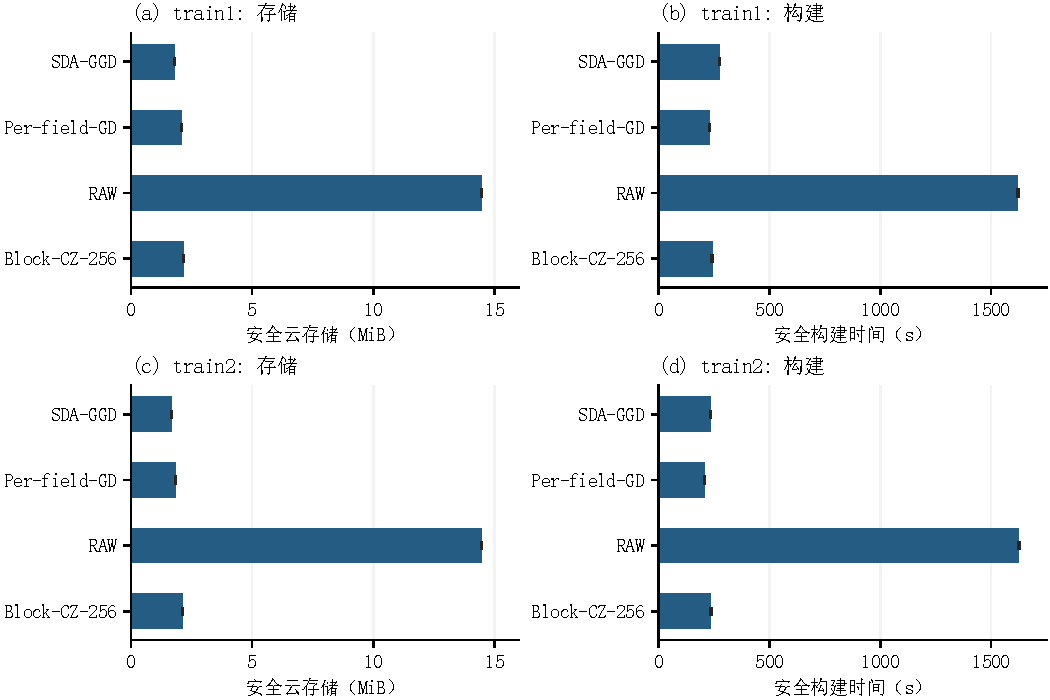
\includegraphics[width=\textwidth]{figures/cn/c1.pdf}
\caption{两个各含 21,600 条记录的 C1 窗口上的云端存储开销与完整构建时间。柱形表示两次构建的中位数，误差线表示观测最小值和最大值。云存储包括密文、审计标签和签名公开清单。}
\label{fig:key-c1}\end{figure*}
\begin{figure*}[t]\centering
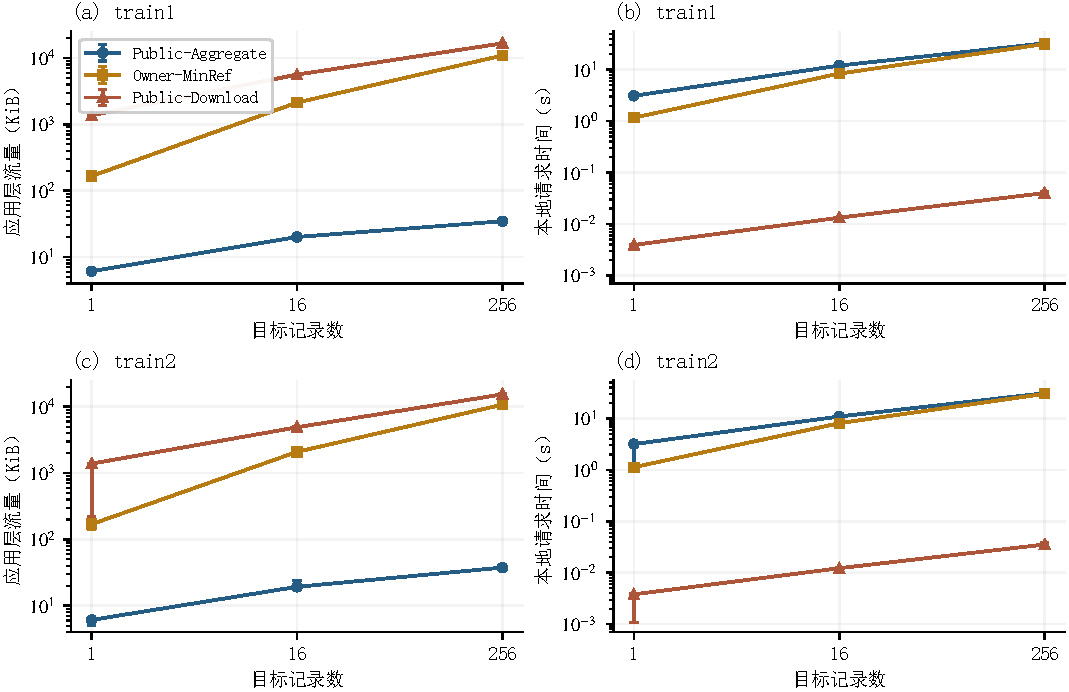
\includegraphics[width=\textwidth]{figures/cn/c2.pdf}
\caption{完整 train1/train2 工作负载上的 C2 应用层流量与完整本地请求时间。每个点表示对应方法和目标数量下三个匹配目标集合的中位数，误差线表示观测范围。Owner-MinRef 持有授权解密能力。初始化单独计量。}
\label{fig:key-c2}\end{figure*}
\begin{figure*}[t]\centering
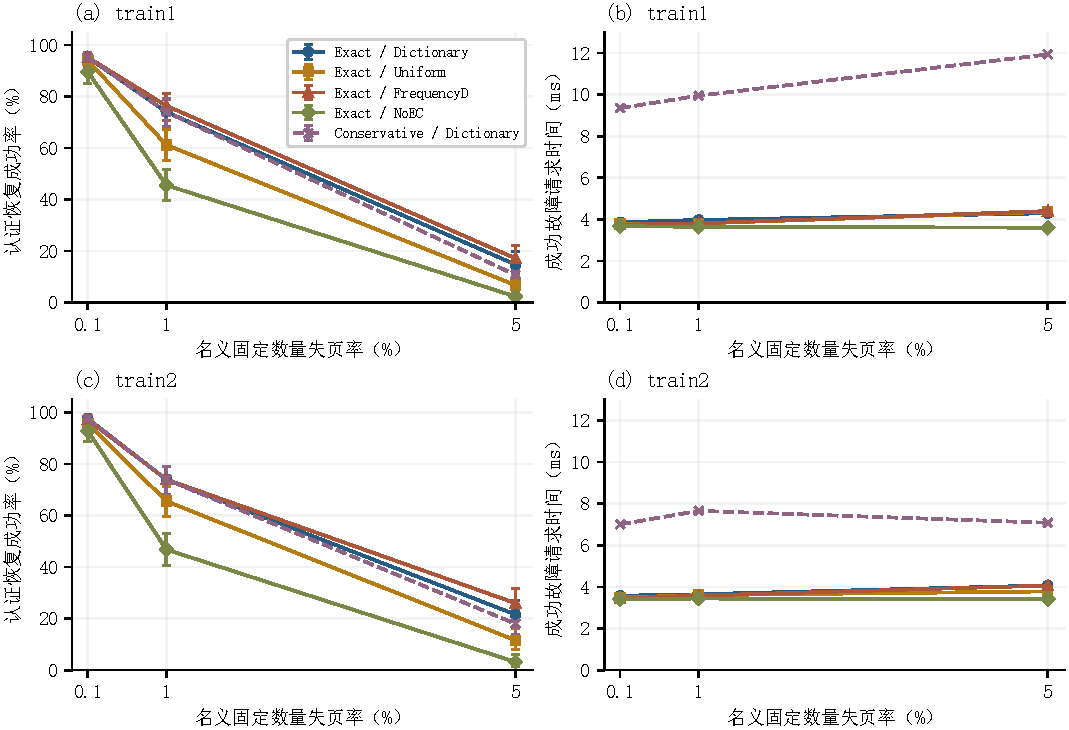
\includegraphics[width=\textwidth]{figures/cn/c3.pdf}
\caption{完整 train1/train2 工作负载上的 C3 单记录认证恢复。成功率点包含五个布局中的 250 个案例，并给出逐点 95\% Wilson 区间。时间点为成功故障请求的中位数。四种 Exact 分配策略与 Conservative/Dictionary 对照区分保护分配和依赖策略。丢失槽位从原始对象与已部署校验槽位构成的共同总体中抽取。受保护排序使用共同条带数量，校验与认证元数据的合计开销以批次密文字节数的 10\% 为上限。}
\label{fig:key-c3}\end{figure*}

\subsection{实验设置}
\subsubsection{数据与实现}
数据源为 HAI 21.03 的 train1 和 train2~\cite{Shin2021HAI}，分别包含 216,001 和 226,801 条记录。原始数据的 84 列由时间、79 个过程字段和四个攻击指示字段组成。三个过程级指示字段独立编码，综合指示字段由其推导。精确十进制规范化保留过程值。每次恢复操作结束后，独立评分器对照规范化源数据检查 $\widehat r_i=r_i$；该检查与客户端的认证及完整解码检查分别进行。

C1 分别选取 train1 中自 2020 年 7 月 11 日 00:00 起和 train2 中自 8 月 1 日 00:00 起的六小时窗口，每个窗口包含 21,600 条记录。C2 和 C3 使用全部记录，train1 划分为三个数据批次，train2 划分为四个数据批次。批次规模和数据源身份见补充材料第~\ref*{supp-sec:key-evidence}~节。每个数据批次独立配置和封装。两者是同一 HAI 数据源下的两个工作负载。下文成对数值均按 train1/train2 顺序给出。

实现使用 Python 3.10.12、NumPy 2.2.6、cryptography 50.0.1 和 py-ecc 8.0.0，组合 AES-256-GCM、Ed25519、BLS12-381 整页认证器与密文 RS$(10,8)$。C1 与完整数据段进程在同一主机上分别绑定 CPU 亲和集合 $\{2\}$ 和 $\{4\}$。输入准备和独立评分位于被测构建或请求操作之外。预置清单与验证者上下文的初始化同请求计时分开。

\begin{table}[t]\centering\small
\caption{评估工作负载与实验单位}\label{tab:scope}
\begin{tabular}{@{}l>{\raggedright\arraybackslash}p{.31\columnwidth}>{\raggedright\arraybackslash}p{.48\columnwidth}@{}}\toprule
内容 & 各数据段记录数 & 对照与观测数量\\\midrule
C1 & 21,600 / 21,600 & 4 种方法，每组构建 2 次；16 次观测\\
C2 & 216,001 / 226,801 & 3 个目标规模、3 个案例、3 类接口；54 次请求\\
C3 & 216,001 / 226,801 & 5 个布局、3 个失页率、50 个案例、8 组对照；12,000 条故障结果\\
无故障 & 同 C3 & 30 个案例、1 个布局、8 组对照；480 条结果\\\bottomrule
\end{tabular}\end{table}

\subsubsection{对照与指标}
C1 比较 SDA-GGD、Per-field-GD、RAW 规范化编码和 Block-CZ-256。Block-CZ-256 在每个含 256 条记录的块内按列序列化非常量字段，并以 Zstd 级别 3 将各块压缩为独立帧。Per-field-GD 用于考察字段分组的作用，RAW 与 Block-CZ-256 提供不同表示方式的对照。所有方法采用相同的安全封装与成本口径。云端字节数包含密文、审计标签和签名公开清单。所有者共享基字节数与总私有磁盘状态分别计量。构建覆盖从规范化输入开始的配置、编码和完整安全封装。

配置样本为 $\min(50{,}000,n)$ 行，在 C1 中等于完整的 21,600 行窗口。该设置评估采用全窗口排序及全量成本确认的分组。每个方法／窗口执行两次，图中报告中位数和观测范围。

C2 分别考察依赖发现方式与响应形式。实验使用 $r=1,16,256$ 个目标，每个数据段／规模使用三个目标集合。Public-Aggregate 接口选择公开闭包；Owner-MinRef-Aggregate（图表中简称 Owner-MinRef）先认证并解密确定精确依赖所需的引用材料；Public-Download 返回公开闭包密文以进行哈希验证。公开接口不使用解密密钥，MinRef 对照具有授权解密能力。Public-Aggregate 与 Public-Download 的比较考察相同公开访问能力下的响应方式；Public-Aggregate 与 Owner-MinRef 的比较进一步考察不同访问能力下的依赖规划。

同一案例中三个接口共享目标。跨批次目标通过各自批次上下文处理。应用层字节数包括声明、挑战、第一阶段材料和响应。完整本地请求时间包括规划及请求接口执行的工作。初始化单独报告；时间轴测量本地处理而非网络传输。每个点报告中位数及最小值至最大值范围。

C3 将 Exact 和 Conservative 恢复分别与 Dictionary、Uniform、FrequencyD、NoEC 四种分配对照组合。固定 Exact 可比较保护分配，固定同一辅助保护文件可比较依赖策略，NoEC 提供零冗余参照。

受保护排序共享 RS$(10,8)$、准入条带数量，以及每批次密文字节数 10\% 的上限，其中计入校验和签名辅助保护状态。FrequencyD 使用每批次前 $\min(4096,\max(1,n/5))$ 条参考记录，$n/5$ 采用整数除法。恢复目标排除这些参考范围。含 7200 条记录的批次使用 1440 条参考记录，其余六个批次各使用 4096 条。评分器仅在服务计时结束后访问源记录；恢复通过云端获取接口和认证修复取得内容。

\subsubsection{故障与统计口径}
对每个数据段，在名义失页比例 $\alpha=0.001,0.01,0.05$ 下评估五个带种子的保护布局，每个布局／失页率包含 50 个案例。每个案例选择一个目标，并从全数据段的原始对象与已部署校验槽位并集中无放回抽取固定数量的丢失槽位。故障总体大小分别为 $N_{\mathrm{fault}}=5000$ 和 $4765$，按 $\lceil\alpha N_{\mathrm{fault}}\rceil$ 得到丢失数量 5/50/250 和 5/48/239。目标在该总体中访问其所属批次。各对照共享目标与槽位丢失掩码；NoEC 使用相应的原始页丢失。策略执行顺序在案例之间轮换。

每个故障成功率点包含全部 250 个结果，并给出以五个被测布局为条件的逐点 95\% Wilson 区间。恢复时间中位数由成功故障请求计算。不同方法的成功集合可能不同，因此需结合成功概率解释时间。无故障恢复在一个布局下对每个数据段／对照运行 30 个案例，共完成 480 次成功的完整记录检查。完整八组结果、失败时延和初始化测量见补充材料。

\subsection{RQ1：存储与安全构建}
在两个窗口上，SDA-GGD 相比 Per-field-GD 均降低云端存储开销（图~\ref{fig:key-c1}）。其存储大小为 1,903,138 和 1,770,118 B，Per-field-GD 则为 2,198,812 和 1,938,839 B，分别降低 13.45\% 和 8.70\%。Block-CZ-256 存储 2,278,001 和 2,227,359 B，RAW 每窗口约为 15.17 MB。全部 16 次构建均通过规范化解码检查。补充材料表~\ref*{supp-tab:key-c1-statistics}~提供字节和计时明细。

存储减少同时带来额外编码工作和较低的标签生成成本。SDA-GGD 完整安全构建的中位时间为 274.356/235.621 s，Per-field-GD 为 231.521/206.163 s，增加 18.50\%/14.29\%。这些比例是观测中位数的描述性比值。SDA-GGD 编码阶段耗时 73.66/47.63 s，Per-field-GD 为 1.00/0.83 s，反映重复组配置与全量成本确认的开销。不过，更少的输出对象将标签生成时间从 230.25/205.05 s 降至 200.42/187.72 s。因此，完整构建成本体现了更多编码工作与更少认证工作的共同作用。

存储表示与所有者侧状态计量不同资源（表~\ref{tab:state}）。SDA-GGD 在 335,884/215,702 B 的总私有状态中保留 303,595/184,687 B 的共享基内容。Per-field-GD 的总状态为 245,064/209,287 B，其中共享基为 208,267/174,552 B。在这两个窗口上，与 Per-field-GD 相比，分组减少了安全云端存储，同时保留了更多所有者侧私有状态。这些测量共同刻画表示与安全构建成本。

\begin{table}[t]\centering\small
\caption{C1 云端与所有者状态}\label{tab:state}
\begin{tabular}{@{}lrrrr@{}}\toprule
& \multicolumn{2}{c}{云端（MiB）} & \multicolumn{2}{c}{所有者（KiB）}\\
方法 & train1 & train2 & train1 & train2\\\midrule
SDA-GGD & 1.815 & 1.688 & 328.012 & 210.646\\
Per-field-GD & 2.097 & 1.849 & 239.320 & 204.382\\
RAW & 14.463 & 14.463 & 0.227 & 0.227\\
Block-CZ-256 & 2.172 & 2.124 & 0.234 & 0.234\\
\bottomrule\end{tabular}
\tabnote{每窗口两次构建的中位数。所有者状态包括共享基目录及私有编码／密钥文件。保护开销单独核算。}
\end{table}

\subsection{RQ2：公开审计的通信与计算}
\emph{相同公开访问能力下的响应。}Public-Aggregate 与 Public-Download 使用相同公开闭包，分别返回聚合证明与密文页（图~\ref{fig:key-c2}）。当 $r=256$ 时，Public-Aggregate 传输 35,405/38,524 B，本地处理耗时 32.532/30.908 s；Public-Download 传输 17,041,940/15,754,868 B，本地处理耗时 0.0400/0.0354 s。聚合认证通过群与域运算减少响应流量，下载接口则支持低成本的本地摘要验证。因此，测得的取舍是以更高的本地处理成本换取更低的应用层流量。本地计时与字节数分别描述两类资源，端到端时间还取决于网络传输。

\emph{不同访问能力下的依赖发现。}公开规划从认证布局获得充分覆盖。Owner-MinRef-Aggregate 先认证并解密引用材料，以缩小最终字典覆盖范围。当 $r=256$ 时，其应用层流量为 11,163,473/11,010,612 B，本地处理耗时 31.532/30.148 s。相较该授权接口，Public-Aggregate 的流量减少 99.68\%/99.65\%，本地处理时间增加 3.17\%/2.52\%。这些百分比是中位数比值，并非配对效应区间。

对于单个目标，Public-Aggregate 耗时 3.106/3.169 s，Owner-MinRef 为 1.164/1.126 s；公开流量为 6237/6254 B，对照为 169,601/173,696 B。引用发现缩小 MinRef 的最终对象覆盖范围，公开规划则省去第一阶段传输。随着目标集扩大，对象重叠和引用并集改变这一平衡。$r=16$ 的点展示中间规模成本；各规模完整数值见补充材料表~\ref*{supp-tab:key-c2-statistics}。

\emph{流量组成。}应用层流量包括请求声明与挑战、需要时传输的第一阶段材料，以及最终响应。当 $r=256$ 时，Owner-MinRef 第一阶段传输的中位数为 11,128,596/10,972,500 B；两种公开接口均无该阶段。两个聚合接口分别为涉及的三个／四个批次返回 12,930/17,240 B 的证明。固定扇区数量下，每个批次贡献 4310 B，声明与挑战随请求变化。补充材料表~\ref*{supp-tab:c2-accounting}~分别给出这些组成部分、服务端读取量与初始化开销。当 $r=1$ 时，所需上下文的初始化时间中位数为 8.101/7.805 s，与上述请求时间分别统计。每个批次上下文初始化一次后复用；这些数值描述请求所需的上下文，而非每次请求重复承担的初始化开销。全部 54 次诚实请求均通过其声明的验证接口。

\emph{机制对照。}两个具有代表性的 16 目标对照分别考察对象复用与聚合。在 train1 批次上，并集读取 805 个对象（3,297,280 B），无缓存分别遍历读取 5643 次（23,113,728 B）；带请求缓存的分别遍历同样读取 805 个对象。相应 train2 对照为 125 次对 892 次无缓存读取，两种带缓存策略均读取 125 次。这说明复用的作用独立于某一种具体遍历方式。

在相同选定页和系数下，聚合证明为 4310 B，而两个对照的逐页证明总大小分别为 3,475,990 B 和 539,750 B。验证时间分别从 472.659 s 降至 3.477 s、从 73.646 s 降至 1.074 s。这些代表性对照解释机制，重复请求实验则提供主要流量与时间曲线。两个对照均拒绝了所测试的末字节密文篡改，该结果与完整密文帧的认证设计一致。

\subsection{RQ3：认证恢复与保护分配}
\emph{保护分配。}固定 Exact 恢复可单独考察保护分配。在共同上限下，Dictionary 相比 Uniform 和 NoEC 提高恢复成功率（图~\ref{fig:key-c3}）。在 1\% 名义失页率下，Dictionary 在两个数据段均恢复 185/250 条记录（74.0\%），Uniform 分别为 153/250 和 164/250（61.2\%/65.6\%），观测差值为 12.8/8.4 个百分点。NoEC 恢复 114/250 和 117/250（45.6\%/46.8\%）。在 0.1\% 下，Dictionary 达到 95.2\%/97.6\%，Uniform 为 94.0\%/95.6\%。

\emph{基于频率的分配。}在 5\% 下，FrequencyD 与 Exact 组合分别成功 43/250 和 65/250（17.2\%/26.0\%），Dictionary 为 14.8\%/21.6\%。在 0.1\% 下，两种策略在 train1 上相同，Dictionary 在 train2 上略高。FrequencyD 优先选择参考记录中频繁使用的依赖对象，Dictionary 则按对象类型确定优先级。在编码、条带数量和预算保持一致时，这些差异说明，保护在记录依赖对象之间的分配方式会影响恢复成功率。补充材料表~\ref*{supp-tab:key-c3-statistics}~保留全部八组对照。

\emph{依赖策略。}固定 Dictionary 辅助保护文件可单独考察恢复所需的依赖。Exact 与 Conservative 在 0.1\% 和 1\% 失页率下具有相同成功结果。在 5\% 下，Exact 恢复 37/250 和 54/250（14.8\%/21.6\%），Conservative 为 27/250 和 45/250（10.8\%/18.0\%）。Exact 在配对案例中分别多成功十次和九次，没有相反方向的失败。当未使用字典对象不可用，而实际记录依赖仍可恢复时，去除前者的可用性要求会产生作用。因此，测得的可用性收益随故障条件和分配策略变化。

\emph{恢复时间。}无故障条件下，Dictionary/Exact 恢复耗时 3.693/3.507 ms，Conservative 为 8.991/7.205 ms。在相同成功目标总体下，精确选择减少了获取和解码的认证内容量。在 5\% 失页率下，成功的 Dictionary/Exact 请求中位时间为 4.298/4.074 ms，Conservative 为 11.933/7.079 ms。这些故障时间中位数包含成功请求的获取及必要修复工作；不同对照的成功总体不同。结合成功率曲线阅读这些结果，可以区分低成本完成与获得完整记录的概率。补充材料表~\ref*{supp-tab:key-c3-time}~在时延旁报告成功数量，完整明细保留失败请求时间。

这些对照揭示两种不同作用：保护分配在同一编码和上限下保护不同共享对象；依赖选择确定目标记录实际需要其中哪些对象。精确认证恢复将两者结合，同时保持相同的密文验证和完整记录接受规则。

\section{结论}
ARC-Audit 通过工业物联网记录到密文对象的认证映射，连接公开审计与认证记录恢复。公开布局提供充分覆盖，经过验证的私有引用确定实际恢复依赖。原始对象与修复对象遵循相同的认证和完整解码规则。实验展示了存储与通信节省及其对应的构建和本地计算成本，也说明保护分配与依赖选择共同决定恢复。当解码器实际需要的认证输入仍可获取时，即使未使用的共享对象不可用，精确选择仍可支持完整记录恢复。

\IEEEtriggeratref{24}
\bibliographystyle{IEEEtran}
\bibliography{IEEEabrv,bstcontrol,references}
\end{document}
